% ********** Device Design Chapter **********
\chapter{Detector Design \& Fabrication}
\label{cha:Design}
\epigraph{`It has long been an axiom of mine that the little things are infinitely the most important.'}{\mbox{\textup{---Sherlock Holmes, The Adventures of}}\\ \mbox{\textup{Sherlock Holmes: A Case of Identity,}}\\ \mbox{\textup{\textsc{Sir Arthur Conan Doyle}}}}
%
\section{Introduction}\label{sec:deisgn_Introduction}
This chapter will detail the design of the silicon cold-electron bolometer detectors studied in this work; it will also look at the process by which these devices have been fabricated. It should, however, be stated at the outset that the designs for these detectors had been arrived at prior to the commencement of this work; as such the process by which the detector design was arrived at will not be covered here. The features of the design will, however, be examined, as will some minor modifications which were added to ensure that the detectors were both functional and relatively simple to fabricate with the facilities available in Cardiff at the time.
%
\section{Detector Design}\label{sec:deviceDesign}
The designed detector was a twin-slot antenna-coupled detector. The absorber (the doped-silicon island of the silicon cold-electron bolometer, described in Chapter~\ref{cha:theory}) was coupled to the antenna via Schottky contacts to the antenna's coplanar waveguide, these Schottky contacts served as the tunnelling contacts to the doped-silicon island, as well as capacitively coupling incident radiation from the antenna via the same waveguide. Since the incident radiation typically has a high frequency ($> 100~\mathrm{GHz}$), it couples directly to the absorber, whereas the bias signal is DC and, as such, must tunnel through the Schottky contacts to reach the absorber, thus producing cooling, as described in Chapter~\ref{cha:theory}. A model of the final detector chip is shown in Figure~\ref{fig:SiCEBchip}.
\begin{figure}[tb]
\begin{center}
\subfloat[]{
	\includegraphics[width=0.45\textwidth]{figures/SiCEBchip}
	\label{fig:SiCEBchip_whole}
}
\subfloat[]{
	\includegraphics[width=0.45\textwidth]{figures/SiCEBchip_zoom}
	\label{fig:SiCEB_zoom}
}
\caption[Model of silicon cold-electron bolometer detector chip]{Model of silicon cold-electron bolometer chip. (a) Whole detector chip with twin-slot antenna; the strained-silicon absorber is located in middle of a coplanar waveguide which is fed by a twin-slot antenna formed in an aluminium ground plane; (b) zoomed-in view of the strained-silicon mesa which acts as the detector's absorber. It should be noted that the height of the strained silicon mesa has been greatly exaggerated here in order to make this component visible. In reality, the silicon substrate is in fact 25,000 times thicker than the mesa.}
\label{fig:SiCEBchip}
\end{center}
\end{figure}
%
\subsection{Antenna Design}\label{ssec:antenna}
A twin-slot antenna was chosen for coupling radiation to the absorber. The reasons for this included the relatively simple design, along with the fact these twin-slot antennae have a linearly-polarised response which allows for signals coupled to the absorber via the antenna to be differentiated from signals due to direct absorption in the strained-silicon mesa. In terms of a detector in an instrument, an antenna with a polarised response clearly allows for the polarisation of a source to be measured.
\par 
\begin{figure}[tb]
\begin{center}
\includegraphics[width = 0.4\textwidth]{figures/twinSlotAntenna_dimensions}
\caption[Key dimensions of a twin-slot antenna]{Key dimensions of a twin-slot antenna.}
\label{fig:twinSlotAntenna_dimensions}
\end{center}
\end{figure}
The key dimensions of a twin-slot antenna are shown in Figure~\ref{fig:twinSlotAntenna_dimensions}. $L$ is the length of the antenna's slots and corresponds to half the wavelength that the antenna is intended to couple to. A caveat to this is that the length corresponds to the wavelength in the medium; in the situation where radiation is coupled to the antenna via a silicon substrate (as indeed was the case in this work), where the refractive index, $n$, is equal to $3.42\mbox{--}3.48$, $L = \nicefrac{\lambda_{0}}{2n} \approx 0.28\lambda_{0}$ where $\lambda_{0}$ is the wavelength in free space. $S$ is the separation between the two slots, this has been optimised via finite-element simulation in Ansoft's HFSS software. $W$ is the width of the slots and is altered to achieve the desired antenna impedance. $a$ and $b$ are the dimensions of the coplanar waveguide and are governed by the desired impedance for the coplanar waveguide.
\par
Three sets of detector design were created, each set had an antenna designed for a different frequency; the selected frequencies were: $160$, $225$ and $360~\mathrm{GHz}$. These frequencies were selected due to their similarity to the second to fifth bands of \textit{Planck}'s \glsfirst{acr:HFI} \parencite[which are $143$, $217$ and $353~\mathrm{GHz}$, as explained by][]{Lamarre2003} used to study the \glsfirst{acr:CMB}. The choice of these antenna frequencies was advantageous due to the wealth of expertise---and indeed equipment---at Cardiff for these frequencies; it also allowed for the potential to access silicon cold-electron bolometers for a possible application (studying the cosmic microwave background). The dimensions (as defined in Figure~\ref{fig:twinSlotAntenna_dimensions}) of these three designs are given in Table~\ref{tab:antennaeDimensions}.
\begin{table}[htb]
\caption[Dimensions of the designed antennae]{Dimensions of the designed antennae.} 
\label{tab:antennaeDimensions}
\centering
\begin{tabular}{S[table-format=3.0]S[table-format=3.0]
										S[table-format=3.0]S[table-format=2.0]
										S[table-format=2.0]S[table-format=2.0]}
\toprule\toprule
{Frequency $\left(\mathrm{GHz}\right)$}&{$L~\left(\mathrm{\upmu m}\right)$}&{$S~\left(\mathrm{\upmu m}\right)$}&{$W~\left(\mathrm{\upmu m}\right)$}&{$a~\left(\mathrm{\upmu m}\right)$}&{$b~\left(\mathrm{\upmu m}\right)$}\\ \midrule
160 & 536 & 333 & 30 & 30 & 58 \\
225 & 356 & 230 & 20 & 30 & 58 \\
360 & 226 & 155 & 15 & 30 & 58 \\
\bottomrule
\end{tabular}
\end{table}
\par
It is clear that if one wishes to either bias or measure (or both) a bridge-type element on the coplanar waveguide, then the design described above, and illustrated in Figure~\ref{fig:SiCEBchip}, has a major flaw: the metal ground plane is contiguous around the twin-slot antenna and is connected directly to the coplanar waveguide; this means that any attempt to measure a resistive component on the coplanar waveguide would be futile, since such a component would be shorted by the ground plane. In order to address this, it was necessary to add cuts to the ground plane such as to force current to be driven through the coplanar waveguide. These were placed on diagonally opposite slots of the antenna, this design is illustrated in Figure~\ref{fig:SiCEBchip_cuts}. While it is clear that these are required for the correct operation of the device, it is fair to say that the placement of these slots was far from optimum since they altered the response of the antenna, this will be seen in greater detail in Section~\ref{sec:antennaSims}. With the gift of hindsight and greater study of literature, it would have been better to have added to slots which extended the coplanar waveguide to one of the edges of the chip \parencite[similar to those described by][]{Focardi2005}.
\begin{figure}[tb]
\begin{center}
\includegraphics[width = 0.6\textwidth]{figures/SiCEBchip_cuts}
\caption[Model of \gls{acr:SiCEB} detector chip with DC cuts in the ground plane]{Model of silicon cold-electron bolometer chip with DC cuts in the ground plane.}
\label{fig:SiCEBchip_cuts}
\end{center}
\end{figure}
\par 
In order for the radiation to be absorbed into the doped-silicon mesa, a break was made in the middle of the coplanar waveguide, where the mesa is situated. The coplanar waveguide overlapped the mesa on both sides and it was at these points that Schottky contacts were formed. This form of structure is often referred to as a bridge, since the bolometer bridges the gap in the coplanar waveguide. This structure, along with the associated dimensions is illustrated in Figure~\ref{fig:twinSlotAntenna_bridge}. 
\begin{figure}[tb]
\begin{center}
\includegraphics[width = 0.4\textwidth]{figures/twinSlotAntenna_bridge}
\caption[Dimensions of bolometer bridge in a coplanar waveguide]{Dimensions of bolometer bridge in a coplanar waveguide. The contact length, $c$, is given by $\nicefrac{\left(y-g\right)\;}{2}$.}
\label{fig:twinSlotAntenna_bridge}
\end{center}
\end{figure}
\par 
Four different values for the contact length, $c$, ($\nicefrac{\left(\mathrm{y-g}\right)\;}{2}$ in Figure~\ref{fig:twinSlotAntenna_bridge}) were selected; these were $1$, $3$, $5$ and $7~\mathrm{\upmu m}$ and were selected not only to allow a study of the effect of varying this parameter but also to help ensure successful fabrication. In all cases, the dimensions $g$ and $x$ were $4$ and $32~\mathrm{\upmu m}$. The anticipated contact resistance for these devices was found based on the contact resistivity, which has been measured for both unstrained and strained doped silicon. The measured values for the contact resistivity, $\rho_{\mathrm{c}}$ were $1.28\times 10^{-4}~\mathrm{\Omega\,cm^{2}}$ for the unstrained doped silicon and $5.12 \times 10^{-3}~\mathrm{\Omega\,cm^{2}}$ for the strained silicon. The dimensions of the bridge were not varied with the different antennae frequencies. The dimensions and expected contact resistance, $R_{\mathrm{c}}$, are given in Table~\ref{tab:bridgeDimensions}.
\begin{table}[htb]
\caption[Dimensions and expected contact resistance for different bolometer bridge designs]{Dimensions and expected contact resistance for different bolometer bridge designs.} 
\label{tab:bridgeDimensions}
\centering
\begin{tabular}{S[table-format=1.0]S[table-format=2.0]S[table-format=2.0]
						S[table-format=2.0]S[table-format=1.0]S[table-format=3.0]
						S[table-format=2.1]}
\toprule\toprule
{}&{}&{}&{}&{}&{Unstrained}&{Strained}\\
{$c~\left(\mathrm{\upmu m}\right)$}&{$x~\left(\mathrm{\upmu m}\right)$}&{$y~\left(\mathrm{\upmu m}\right)$}&{$a~\left(\mathrm{\upmu m}\right)$}&{$g~\left(\mathrm{\upmu m}\right)$}&
{$R_{\mathrm{c}}~\left(\mathrm{\Omega}\right)$}&{$R_{\mathrm{c}}~\left(\mathrm{k\Omega}\right)$}\\ \midrule
1 & 32 & 6 & 24 & 4 & 533 & 21.3 \\
3 & 32 & 10 & 24 & 4 & 178 & 7.1 \\
5 & 32 & 14 & 24 & 4 & 107 & 4.3 \\
7 & 32 & 18 & 24 & 4 & 76 & 3.0 \\
\bottomrule
\end{tabular}
\end{table}
%
\section{Detector Fabrication}\label{sec:fabrication}
The detector chips were fabricated via sputter deposition and photolithographic techniques. In order for the devices to be fabricated, a photomask was created. This mask was used for the two steps in the fabrication process which required etching of a material (covered later in this section); an example of two sections of this mask, used to a create a single detector, is shown in Figure~\ref{fig:photomask}. In this figure, features in black are those protected from the etching process and are those present on the final detector chip. In Figure~\ref{fig:photomask_step1}, this corresponds to doped silicon whereas in Figure~\ref{fig:photomask_step2}, this corresponds to aluminium.
\begin{figure}[tb]
\begin{center}
\subfloat[]{
	\includegraphics[width=0.35\textwidth]{figures/photomask_step1}
	\label{fig:photomask_step1}
}\hspace{0.1\textwidth}
\subfloat[]{
	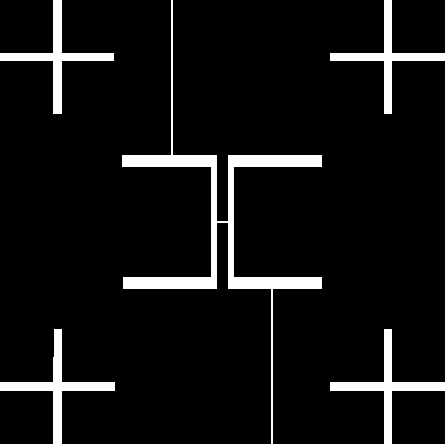
\includegraphics[width=0.35\textwidth]{figures/photomask_step2}
	\label{fig:photomask_step2}
}
\caption[Example sections from photomask]{Example sections from the photomask used to fabricate silicon cold-electron bolometers. (a) First step, creation of the absorbing mesa; (b) second step, creation of the twin-slot antenna structure. In both stages, the features on the mask in black were protected from the etching process and thus were present on the final detector chip. The features in the corners are alignment marks used to align the mask during the second stage.}
\label{fig:photomask}
\end{center}
\end{figure}
\par 
The fabrication process itself is relatively simple, containing only three etching steps and a single deposition step. The full process flow for the fabrication of the detectors tested in this work is given in the following points:
\begin{description}
\item[Initial wafer] The starting wafers have been grown at The University of Warwick and have been detailed by \textcite{Muhonen2011}. The wafers consist of a silicon (001) substrate, followed by a $30~\mathrm{nm}$ layer of epitaxial n\textsuperscript{++} silicon in the case of the unstrained silicon. In the case of the strained silicon, a $2~\mathrm{\upmu m}$ graded layer of \ce{Si_{$1-x$}}\ce{Ge_{$x$}} is grown on top of the substrate; this layer is linearly graded from $x=0$ at the interface to $x=0.2$. This layer is followed by a $500~\mathrm{nm}$ layer of \ce{Si_{0.8}}\ce{Ge_{0.2}}. Finally a $30~\mathrm{nm}$ layer of n\textsuperscript{++} silicon is grown on top of the \ce{SiGe}.
\item[Mesa defined] The mesa structure (the absorber) is defined with photoresist. This is applied evenly to the wafer and briefly baked to ensure all excess liquid is removed. The first stage of the photomask (Figure~\ref{fig:photomask_step1}) is then placed over the wafer and the photoresist is exposed to ultraviolet light through the photomask. Parts of the mask which are solid (those which are black in Figure~\ref{fig:photomask}) block the ultraviolet light, protecting the photoresist. The photoresist which has been exposed is weakened and removed with a developer solution.
\item[Mesa etching] The mesa structure is created via etching away the undesired parts of the doped-silicon layer. The etching process is unable to etch through the photoresist and thus only the regions exposed to ultraviolet light in the previous step are etched. For the creation of silicon cold-electron bolometers, this etching was performed with a \ce{CF_{4}}/\ce{O_{2}} gas etch. The parameters for this etch were: $30~\mathrm{sccm}$ at a pressure of $50~\mathrm{mBar}$ and a power of $100~\mathrm{W}$.
\item[Surface preparation] During early testing of junctions, it was found that in order to create a high-quality Schottky barrier, it was vital to remove the thin layer of silicon oxide (\ce{SiO_{2}}) which formed on the doped silicon during storage of the wafer and the above steps. This was performed by briefly etching the wafer in a weak aqueous solution of hydrofluoric acid. This process removed the silicon oxide layer and left hydrogen-terminated silicon at the surface, preventing re-oxidisation of the wafer.
\item[Aluminium deposition] The aluminium---which created the contacts to the doped-silicon absorber, as well as the ground plane for the antenna---was deposited via sputter deposition. This was performed at a pressure of $5 \times 10^{-3}~\mathrm{mBar}$ and a sputter power of $150~\mathrm{W}$. The sputtering gas used was Argon.
\item[Antenna defined] The antenna pattern was defined with the second stage of the photomask (Figure~\ref{fig:photomask_step2}) and the same process as described above for the mesa.
\item[Antenna etching] The antenna structure was etched using a wet etching solution consisting of 26 parts \ce{HPO_{3}}, 6 parts \ce{H_{2}O} and 2 parts nitric \ce{HNO_{3}}. The final aluminium layer was approximately $100~\mathrm{\upmu m}$ thick.
\end{description}
\begin{figure}[tb]
\begin{center}
\subfloat[]{
	\includegraphics[width=0.35\textwidth]{figures/CEB_structure}
	\label{fig:CEB_crossSection}
}\hspace{0.1\textwidth}
\subfloat[]{
	\includegraphics[width=0.35\textwidth]{figures/CEB_structure_strained}
	\label{fig:CEB_crossSection_strained}
}
\\
\subfloat[]{
	\includegraphics[width=0.6\textwidth]{figures/CEB_photograph}
	\label{fig:CEB_photograph}
}
\caption[Cross sections of strained and unstrained \gls{acr:SiCEB} structures and photograph of a fabricated detector]{(a) Cross section of an unstrained \gls{acr:SiCEB} detector. (b) Cross section of a \gls{acr:SiCEB} detector with a strained-silicon absorber. Both cross sections are along the axis of the coplanar waveguide. (c) Optical photograph of a silicon cold-electron bolometer.}
\label{fig:CEB_crossSection_photograph}
\end{center}
\end{figure}
\par
The process above was used for the fabrication of all devices. The cross sections of the two types of detector fabricated (those with and without a strained absorber) are shown in Figure~\ref{fig:CEB_crossSection_photograph}, along with a photograph (taken using a microscope) of one of the fabricated devices.
%
\section{Material Properties}\label{sec:materialProperties}
As has been mentioned previously in this chapter, two different silicon wafers have been used to fabricate silicon cold-electron bolometers. These were an unstrained highly-doped silicon (sometimes referred to in literature as the \textit{control} material, wafer reference number: 5365) and a strained highly-doped silicon (wafer reference number: 5362). A detailed study of these two materials has been presented by \textcite{Muhonen2011} but a summary of the key properties of these two materials is given in Table~\ref{tab:materialProperties}.

\begin{table}[htb]
\caption[Summary of key material properties for unstrained (control) and strained silicon materials]{Summary of key material properties for unstrained (control) and strained silicon materials.} 
\label{tab:materialProperties}
\centering
\begin{threeparttable}
\begin{tabular}{lcc}
\toprule\toprule
{Parameter}&{Unstrained}&{Strained}\\
\midrule
Dopant Concentration $\left(\mathrm{cm}^{-3}\right)$ \tnote{a} & $4\times 10^{19}$ & $4\times 10^{19}$  \\[1.1ex]
Strain Layer \tnote{a} & {N/A} & {\ce{Si_{0.8}Ge_{0.2}}}  \\[1.1ex]
Carrier Density $\left(\mathrm{cm}^{-3}\right)$ \tnote{a} & $3.1\times 10^{19}$ & $2.7\times 10^{19}$ \\[1.1ex]
Mobility $\left(\mathrm{cm}^{2}\,\mathrm{V}^{-1}\,\mathrm{s}^{-1}\right)$ \tnote{a} & 192 & 155 \\[1.1ex]
Electron-Phonon Coupling, $\varSigma$ $\left(\mathrm{W\,K}^{-6}\,\mathrm{m}^{-3}\right)$ \tnote{b} & $5.2\times 10^{8}$ & $2.0\times 10^{7}$ \\[1.1ex]
Sheet Resistance $\left(\mathrm{\Omega/\square}\right)$ & 384  & 571 \\[1.1ex]
Al-Si Junction Resistance $\left(\mathrm{k\Omega\,\upmu m}^{2}\right)$ & 13 & 512\\
\bottomrule
\end{tabular}
\begin{tablenotes}
\item[a] From \textcite{Muhonen2011}.
\item[b] From \textcite{Prest2011}.\\
The sheet resistance and aluminium-silicon junction resistance have been measured at Cardiff.
\end{tablenotes}
\end{threeparttable}
\end{table}

